An overview of the aggregated molecule information can be seen in
the table view. All the molecule properties, as well as their titles,
SVG-images and the flags set by users, are shown in form of a table.
%
\begin{figure}[!htb]
\begin{centering}
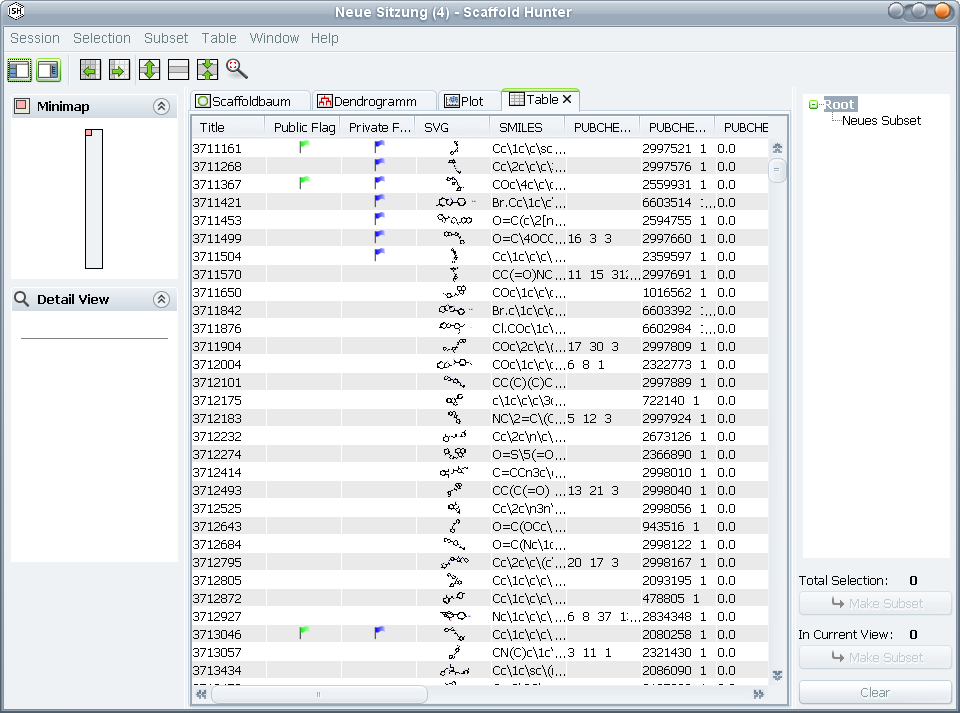
\includegraphics[width=0.8\columnwidth]{images/table/table_overview}
\par\end{centering}

\caption{The tableview}


%
\end{figure}



\subsection{Sorting and Ordering the Table}

When you open a table view the data is initially sorted by the molecule
title, but the sort order can be changed anytime by clicking on a
column header. The table view supports three sort criteria, which are
applied by consecutive clicks on column headers. The column selected last
gets the highest sort priority.

Apart from sorting the rows of the table you can reorder the columns
at any time by dragging them to their new position.


\subsection{Resizing Table Cells}

A table cell is often too small to show the information that it holds.
In this case three little dots appear at the end of the cell, to indicate
that the content is not completely shown. To address this problem there
are two ways to resize table cells: To change the width of a column
you can simply click on the right boundary line of the column header
and move it to the left or right, to make the whole column smaller
or wider. The height of the rows can be changed via three buttons
in the \tbar:
\begin{itemize}
\item 
\includegraphics{images/table/table_lines_enlarge} the
\textit{increase} button allows you to increase the number of text lines
that are shown in a table cell. Each time it is clicked one more line
is added.
\item 
\includegraphics{images/table/table_lines_shrink} the
\textit{decrease} button decreases the number of text lines per cell. 
\item 
\includegraphics{images/table/table_lines_normalize} the
\textit{normalize} button sets the number of text lines back to the
default value of one.
\end{itemize}
The content of a table cell is also shown in the \textit{Detail View}
panel in the \sbar, as soon as you move the mouse pointer to a cell.

%
\begin{figure}[!htb]
\begin{centering}
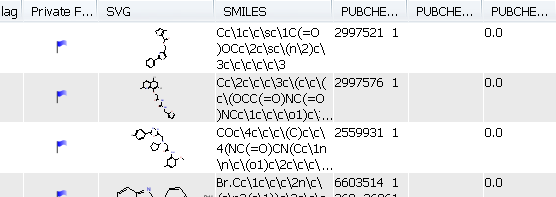
\includegraphics[width=0.8\columnwidth]{images/table/table_rowheight_example}
\par\end{centering}

\caption[Enlarged table rows]{Example of a table that shows three text lines in a table cell}


%
\end{figure}



\subsection{The Minimap}

The Minimap shows an abstract view of the complete table, where the
section that is currently shown in the main view is highlighted in
light red. Apart from just informative reasons the minimap can also
be used to scroll the table. Just click on the highlighted box and
drag it to another position.


\subsection{Sticky Columns}

When the table holds a lot of columns -- which is a very common case
-- then it is eligible that some columns are not scrolled horizontally
but stay visible the whole time. The molecule title column is an example;
it may be helpful if this column is always visible. This can be accomplished
by putting table columns into the \textit{sticky mode}: A sticky column
does not scroll horizontally. 

This feature can be accessed by two buttons in the \tbar:
\begin{itemize}
\item 
\includegraphics{images/table/table_sticky_add} A
click on this button turns the leftmost floating column (a column
which is not yet sticky) into the sticky mode. It will not scroll
horizontally anymore.
\item 
\includegraphics{images/table/table_sticky_remove} This
button turns the rightmost sticky column back into floating mode,
which means that the column will scroll as usual.
\end{itemize}
To indicate that a column is sticky it is shown a bit darker than
a normal, floating column.

%
\begin{figure}[!htb]
\begin{centering}
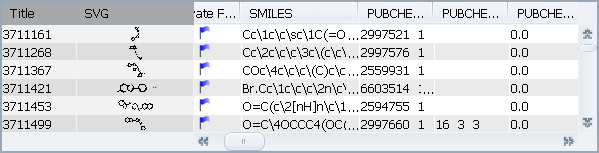
\includegraphics[width=0.8\columnwidth]{images/table/table_sticky_example}
\par\end{centering}

\caption[Sticky columns]{A table with two sticky columns. Note that the scrollbar at the bottom
does not include the sticky columns.}


%
\end{figure}



\subsection{Setting Flags}

Flags (public and private) can be set by using the context menu that
appears when you right-click anywhere in the table. The menu item ``Toggle
public flag (for \textit{molecule title})'' lets you toggle the public
flag for the specified molecule. The item ``Toggle private flag
(for \textit{molecule title})'' does the same for private flags. The
flags are shown in the table in separate columns.


\subsection{Selecting Molecules}

The selection of molecules (a row in the table) works slightly different
than with common tables. The only change we made is that the current
selection will not be cleared when you select a new molecule by clicking
on the corresponding row in the table. So you can select/unselect
multiple molecules by consecutive clicking on them.

Additionally you can select many molecules in a row when you hold
down the \texttt{Shift} key while clicking on the first and the last
molecule you want to select (which is the common behavior that you
may know from other programs).


\subsection{Writing and Editing Comments}

The comment editor for molecules can be opened by using the context menu. 


\subsection{Placeholders in Table Cells}

The table can be used to access all molecule information which is
stored in the database. To conserve memory these information are loaded
just when they should be shown. This may cause a little delay in
displaying the content of the table, which can be noticed at fast
scrolling over a long distance. During the loading process the table cells
are filled with three dots ({}``\ldots{}'') as placeholders. These
placeholders are replaced by the real content as soon as it is available.
